\section{Цель работы}
\begin{enumerate}
    \item Измерение модуля ускорения свободного падения.
    \item Экспериментальная проверка эквивалентности гравитационной
        и инертной массы
\end{enumerate}

\section{Задачи}
\begin{enumerate}
    \item Измерение времени движения тележки по рельсу при разных
        углах наклона рельса к горизонту.
    \item Исследование зависмости ускорения тележки от угла наклона
        рельса к горизонту. Определение ускорения свободного падения.
\end{enumerate}

\section{Объект исследования}
Объект исследования - ускорение гравитационного падения.

\section{Метод экспериментального исследования}
Многократное прямое измерение ускорения тележки при прохождении определенного
расстояния под определенным углом к горизонту.

\section{Рабочие формулы и исходные данные}
\begin{enumerate}
    \item $ \sin \alpha = \frac{(h'_0 - h') - (h_0 - h)}{x' - x} $ --- синус угла наклона тележки к горизонту
    \item $\langle a \rangle = \frac{\sum_{i=1}^N a_i}{N}$ --- среднее значение ускорения
    \item $\sigma_a = \sqrt{\frac{\sum_{i=1}^N (a_i - \langle a \rangle)^2 }{N - 1}}$ --
        стандартное отклонение отдельного измерения
    \item $ \Delta a = \frac{\alpha_{0.95, N} \cdot \sigma}{\sqrt{N}} $ -- погрешность измерений
    \item
        $ B = \frac{ \sum_{j=1}^n a_j \sin(\alpha)_j -
        \frac{1}{n} \sum_{j=1}^n a_j \sum_{j=1}^n \sin(\alpha)_j}{\sum_{j=1}^n \sin^2(\alpha)_j - \frac{1}{n} (\sum_{j=1}^n \sin(\alpha)_j)^2} $
        $ A = \frac{1}{n} \left( \sum_{j=1}^n a_j - B \sum_{j=1}^n \sin(\alpha)_j \right) $
        --- коэфиициенты линейной зависимости по методу наименьших квадратов
    \item $\sigma_B = \sqrt{\frac{\sum_{j=1}^n d_j^2}{D(n-2)}}$ --- стандартное отклонение
        для коэффициента $B$, где $d_j = a_j - (A + B \sin (\alpha)_j)$,
        $D = \sum_{j=1}^n \sin^2(\alpha)_j - \frac{1}{n} (\sum_{j=1}^n \sin(\alpha)_j)^2$ 
    \item $\Delta B = 2 \sigma_B$, $\varepsilon_B = \frac{\Delta B}{B} \cdot 100\%$ --- абсолютная
        и относительная погрешность для доверительной вероятности $0.9$.
        
\end{enumerate}

\section{Измерительные приборы}
\begin{table}[ht]
    \begin{tabular}{| c | c | c | c | c |}
        \hline
        \textnumero п/п & Наименование & Тип прибора & Используемый диапазон & Погрешность \\
        \hline
        1 & Угольник & Аналоговый & 0-20 см & 0.1 см \\
        \hline
        2 & Программа SPARKVUE & Цифрвоой & $0.01 - 0.03 \, {\text{м}}/{\text{с}^2 }$ & $0.0001 \, {\text{м}}/{\text{с}^2 }$ \\
        \hline

    \end{tabular}
    \caption{Измерительные приборы}
\end{table}

\section{Схема установки}
\begin{figure}[ht]
    \centering
    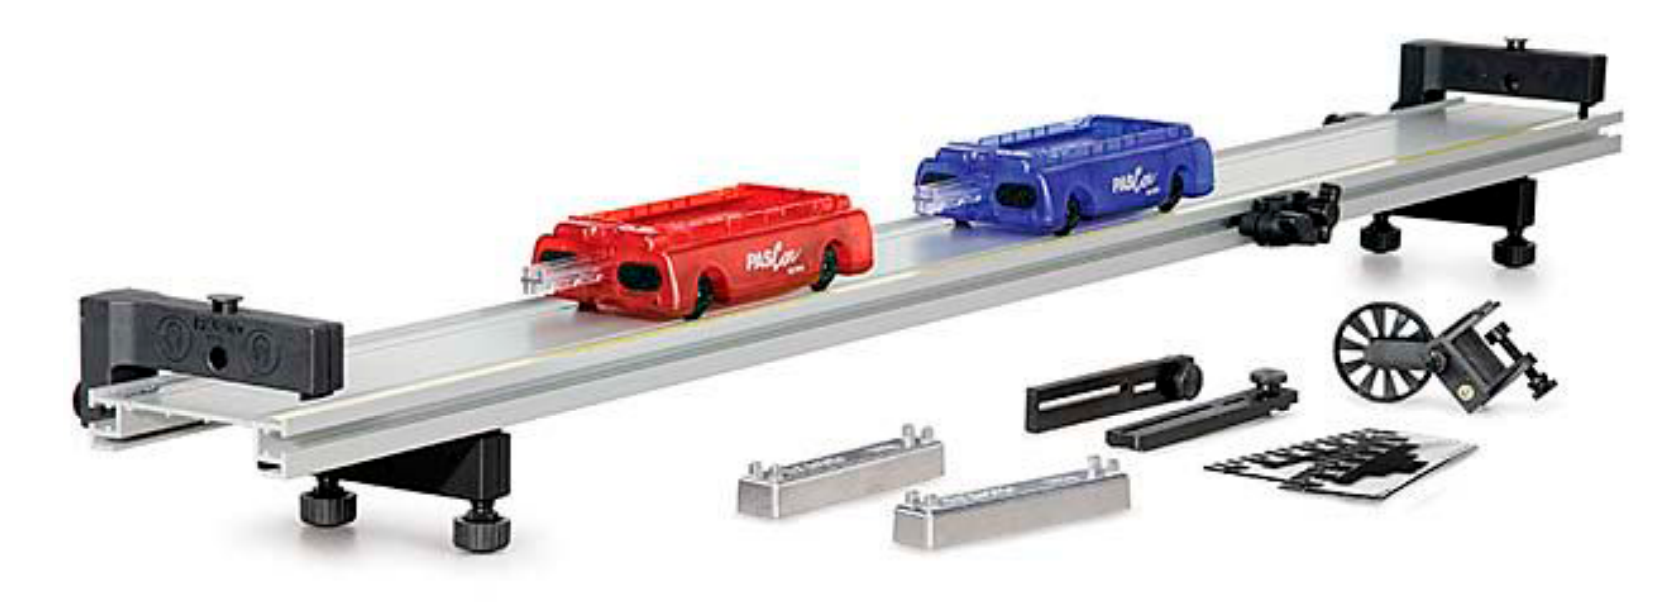
\includegraphics[width=\textwidth]{img/scheme.png}
    \caption{Схема установки}
\end{figure}
